% ===================================================================
% Presentación con Latex Beamer
% ===================================================================
\documentclass[10pt,xcolor=svgnames]{beamer}
% \documentclass[handout,xcolor=svgnames]{beamer} %Version imprimible
% -------------------------------------------------------------------
% Paquetes personalizados
\usepackage{paquetes}
\usepackage{colores}
\usepackage{info}
\usepackage{modo}
\usepackage{licencia}
% -------------------------------------------------------------------

% Comienza el documento
\begin{document}
% Tikz -> Imágenes
%\tikzstyle{every picture}+=[remember picture]
% Entorno matemático
\everymath{\displaystyle}
% ------------------------------------------------------------------

% Título a partir del fondo especial
\begin{frame}
  \maketitle
\end{frame}

% Transparencia de índice
\begin{frame}{Índice}
  \tableofcontents
\end{frame}

\section{Introducción}


\subsection{Contexto}

\begin{frame}{¿Por qué este proyecto?}
  \begin{block}{Cuando cocinamos...}
    \begin{itemize}
    \item leemos las recetas desde el dispositivo
    \item paramos para ver cada paso
    \item podemos poner en riesgo el dispositivo
    \end{itemize}
  \end{block}

  \begin{center}
    Motivación personal
  \end{center}
\end{frame}

\subsection{Objetivos}

\begin{frame}{Objetivos}
  \begin{center}
    Crear una aplicación móvil de acceso \textbf{público} que permita la
    visualización de \textbf{recetas} de cocina
  \end{center}

  \vspace*{0.5cm}

  \textsc{Requisitos:}\\
  \begin{enumerate}
  \item Lectura automática y captura de órdenes
  \item Creación y subida de recetas
  \item Categorización y filtrado (alérgenos)
  \item Multiidioma
  \end{enumerate}
\end{frame}


\begin{frame}{¿Por qué Android?}  
  \begin{block}{Android}
    Sistema operativo basado en el núcleo Linux
  \end{block}
  

  
  \begin{minipage}[t]{.6\textwidth}
    \vspace*{0.3cm}
    \begin{itemize}
    \item Popularidad
    \item Interés personal (iOS descartado)
    \item Biblioteca \textsc{Text To Speech}
    \item Biblioteca \textsc{Speech Recognizer}
    \end{itemize}
  \end{minipage}%
  \begin{minipage}[t]{.4\textwidth}    
    \begin{figure}[H]
      \centering
      
\includegraphics[width=\textwidth]{./img/android-logo}
    \end{figure}
  \end{minipage}
\end{frame}

\begin{frame}{¿Por qué Django?}  
  \begin{block}{Django}
    Framework de desarrollo web basado en MVC
  \end{block}
  
  \begin{minipage}[t]{.6\textwidth}
    \vspace*{0.5cm}
    \begin{itemize}
    \item Python en desarrollo web
    \item Popularidad
    \item Robustez
    \item Software libre
    \item Django Rest Framework
    \end{itemize}
  \end{minipage}%
  \begin{minipage}[t]{.4\textwidth}    
    \begin{figure}[H]
      \centering
      
\includegraphics[width=\textwidth]{./img/python-y-django}
    \end{figure}
  \end{minipage}
\end{frame}


\subsection{Planificación}

\begin{frame}{Desarrollo iterativo}

  \begin{enumerate}
  \item Preparación previa:
    \begin{itemize}
    \item Definición de requisitos y planificación
    \item Aprendizaje autodidacta
    \item Diseño visual
    \end{itemize}
  \item Desarrollo de la base de la API
  \item Desarrollo de la base de la app
  \item Ampliación de la API
  \item Amplicación de la app
  \item Revisión
    \begin{itemize}
    \item Despliegue en producción de la API
    \item Plan de pruebas - testers
    \item Resolución de \textit{bugs}
    \item Documentación
    \end{itemize}
  \end{enumerate}
  
\end{frame}
  
\begin{frame}{Estimación VS tiempo real}
  \begin{cambiarmargen}{-2.5cm}{-2.5cm}

    \begin{table}[hbtp]
      \centering
      \begin{tabular}{|l|r|r|}
        \hline
        \textbf{Iteración} & \textbf{Tiempo estimado} & \textbf{Tiempo real} \\
        \hline
        Planificación & 56 horas & \textcolor{red}{77 horas} \\
        \hline
        Aprendizaje & 224 horas & \textcolor{red}{242 horas} \\
        \hline
        Diseño visual & 56 horas & \textcolor{verde}{22 horas} \\
        \hline
        Desarrollo API & 128 horas & \textcolor{verde}{110 horas} \\
        \hline
        Desarrollo app & 128 horas & \textcolor{red}{132 horas} \\
        \hline
        Ampliación API & 168 horas & \textcolor{verde}{88 horas} \\
        \hline
        Ampliación app & 216 horas & \textcolor{red}{222 horas} \\
        \hline
        Despliegue & 32 horas & \textcolor{verde}{26 horas} \\
        \hline
        Resolución de \textit{bugs} & 160 horas & \textcolor{verde}{152 horas} \\
        \hline
        Documentación & 80 horas & \textcolor{verde}{65 horas} \\
        \hline
        \textbf{Total} & 1249 horas & \textcolor{verde}{1136 horas} \\
        \hline
      \end{tabular}
      \label{tab:estimacion_tiempo}
    \end{table}
    
  \end{cambiarmargen}
\end{frame}


%% Contenido

\section{El proyecto}

\subsection{Descripción}

\begin{frame}{¿Qué es Amuse Bouche?}

  \begin{figure}[H]
    \centering
    
\includegraphics[width=0.3\textwidth]{./img/logotipo}
  \end{figure}

  \begin{center}
    API + Aplicación móvil
  \end{center}
  
\end{frame}

\begin{frame}{API}

  API REST para manejar los datos a compartir:
  
  \begin{itemize}
  \item Usuarios
  \item Recetas
    \begin{itemize}
    \item Categorías
    \item Ingredientes
    \item Pasos      
    \end{itemize}
  \item Puntuaciones
  \item Comentarios
  \end{itemize}

  Y los datos para funcionalidades extra:
  \begin{itemize}
  \item Ingredientes categorizados
    \begin{itemize}
    \item Categorías
    \item Traducciones
    \end{itemize}
  \end{itemize}
  
\end{frame}

\begin{frame}{Aplicación móvil}
  \begin{itemize}
  \item Funcionalidad:
    \begin{itemize}
    \item Crear y editar recetas a nivel local
    \item Compartir recetas
    \item Lectura automática y captura de órdenes
    \item Multiidioma
    \item Categorización y filtrado
    \end{itemize}
  \item Funcionalidades y detalles extra:
    \begin{itemize}
    \item Material Design
    \item Modo sin conexión
    \item Modo solo WiFi
    \item Autocompletado de ingredientes (en filtrado y añadir ingrediente)
    \item Cronómetro integrado
    \end{itemize}
  \end{itemize}
\end{frame}

\begin{frame}{Aplicación móvil}
  \begin{minipage}{\linewidth}
    \centering
    \begin{minipage}{0.4\linewidth}
      \begin{figure}[H]
        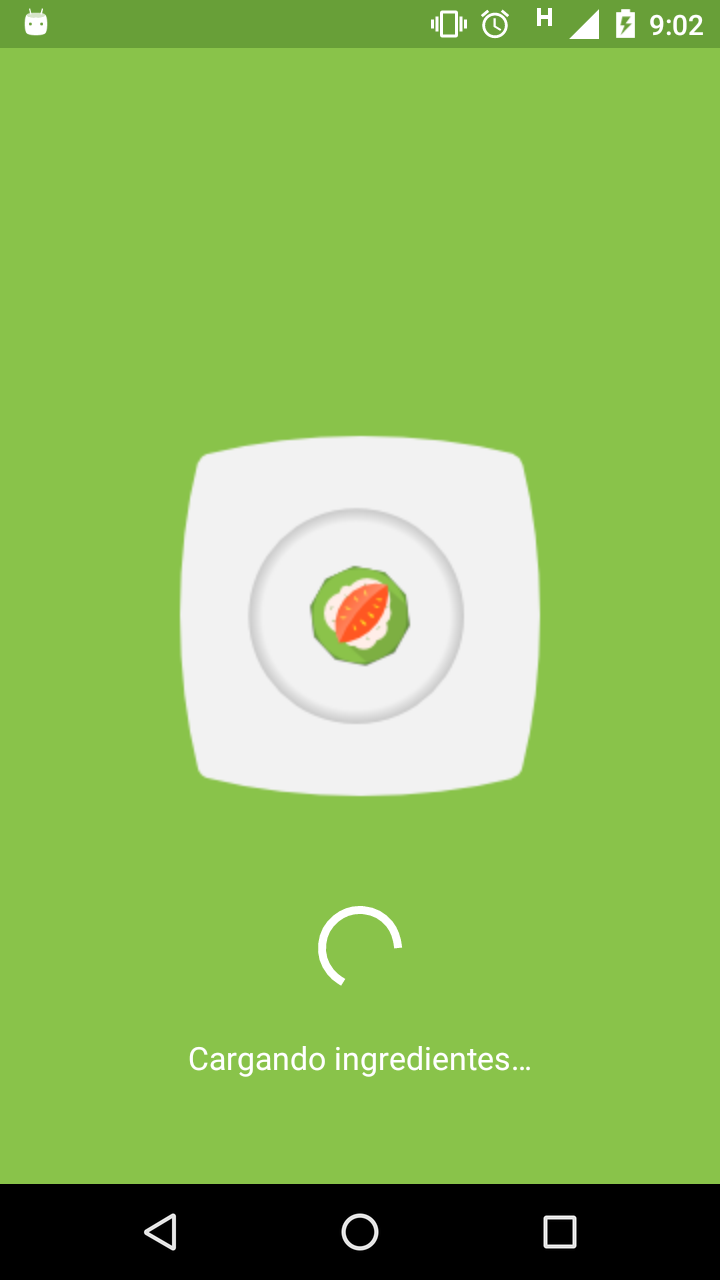
\includegraphics[width=\linewidth]{img/captura_02}
      \end{figure}
    \end{minipage}
    \hspace{0.05\linewidth}
    \begin{minipage}{0.4\linewidth}
      \begin{figure}[H]
        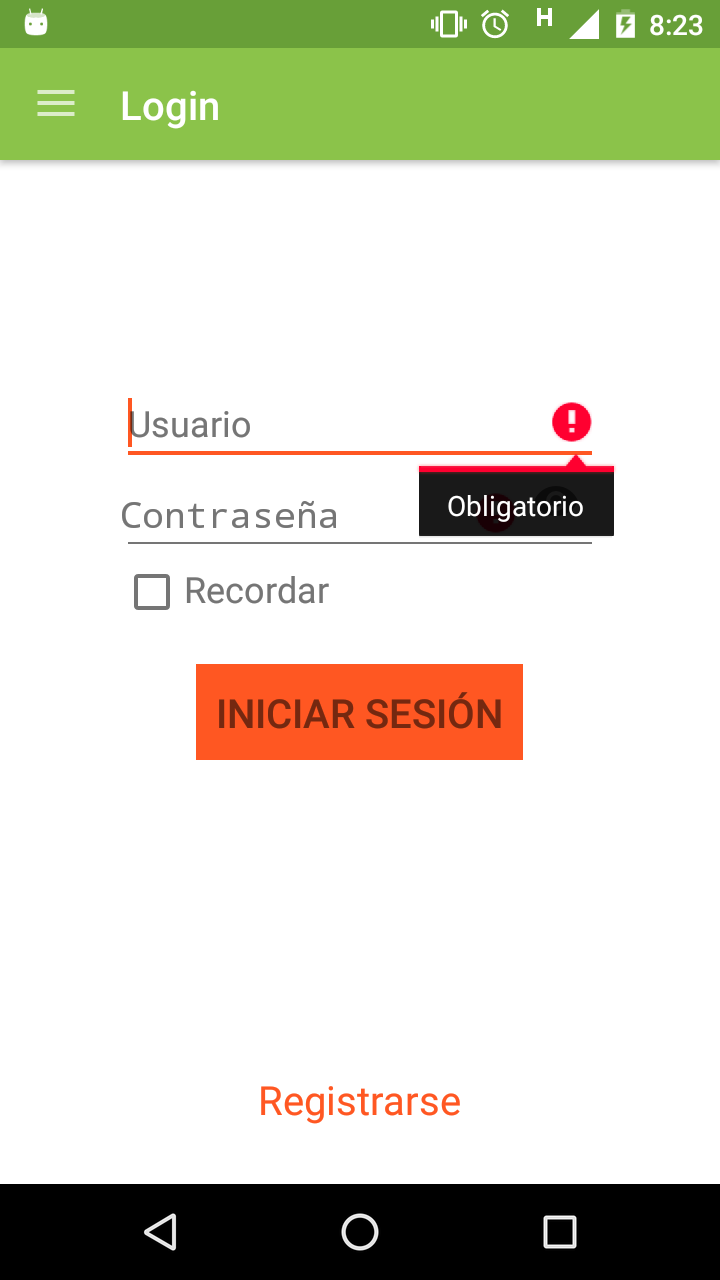
\includegraphics[width=\linewidth]{img/captura_13}
      \end{figure}
    \end{minipage}
  \end{minipage}
\end{frame}

\begin{frame}{Aplicación móvil}
  \begin{minipage}{\linewidth}
    \centering
    \begin{minipage}{0.4\linewidth}
      \begin{figure}[H]
        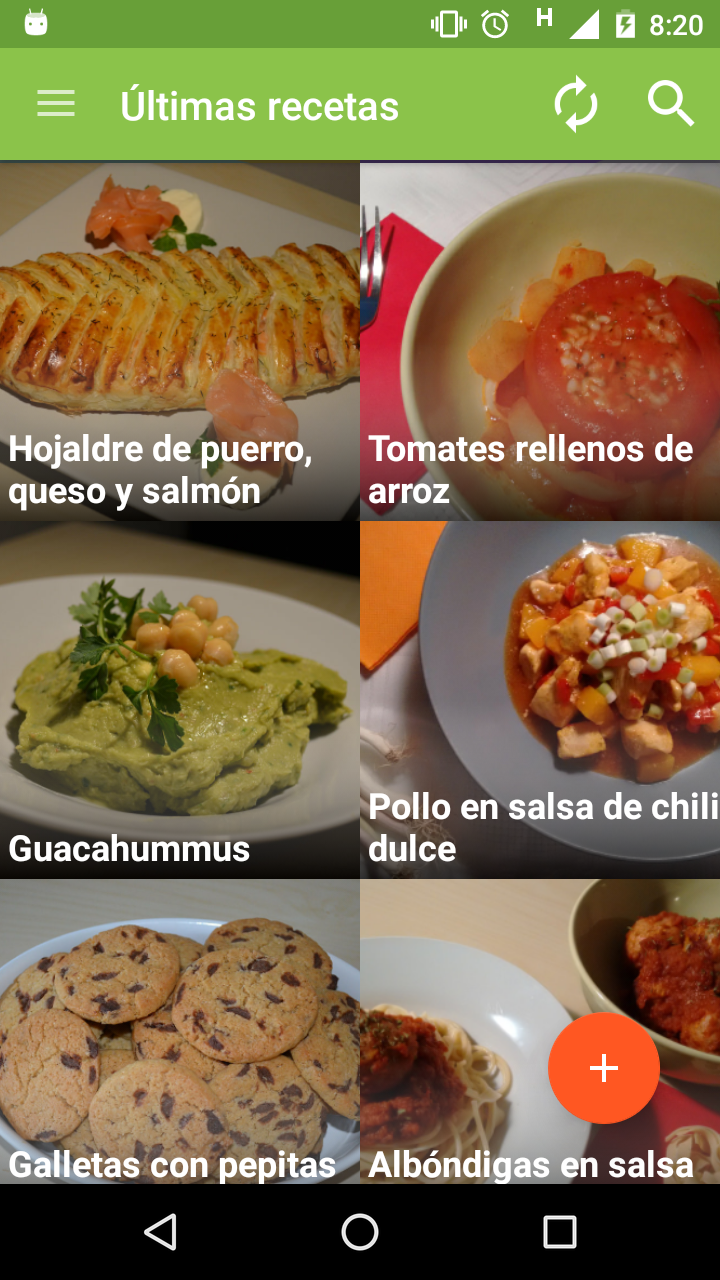
\includegraphics[width=\linewidth]{img/captura_03}
      \end{figure}
    \end{minipage}
    \hspace{0.05\linewidth}
    \begin{minipage}{0.4\linewidth}
      \begin{figure}[H]
        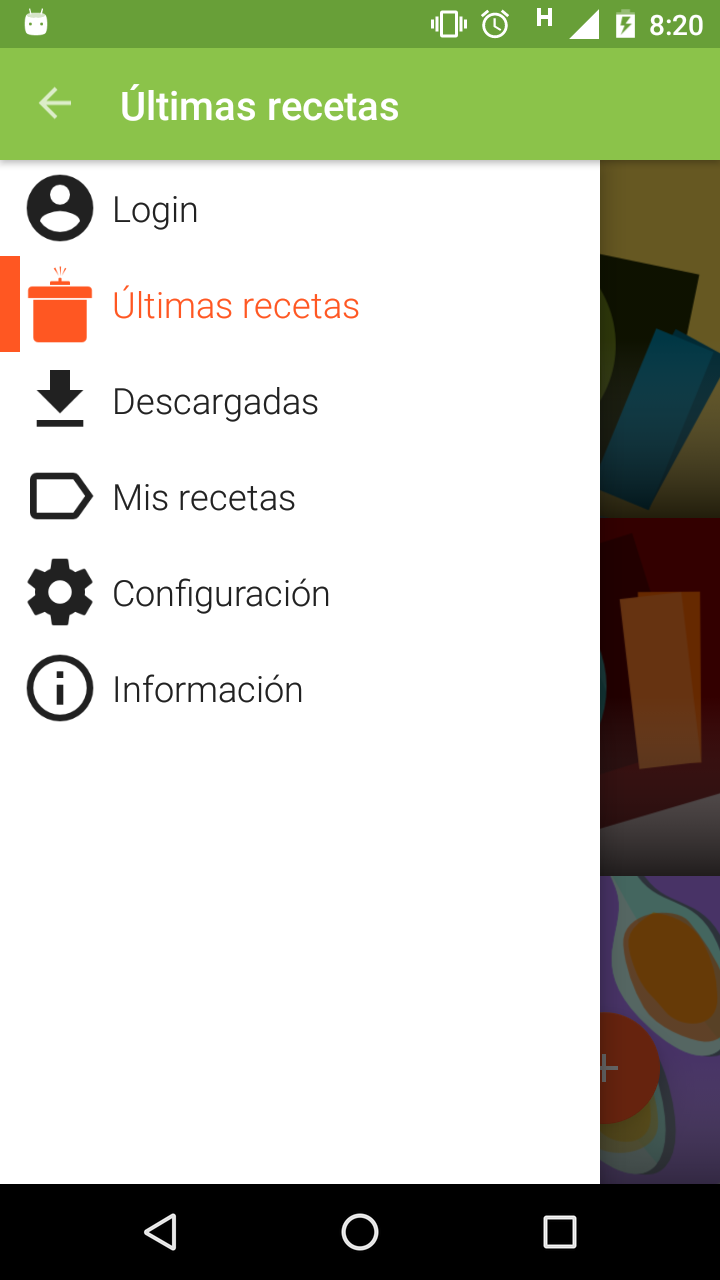
\includegraphics[width=\linewidth]{img/captura_05}
      \end{figure}
    \end{minipage}
  \end{minipage}
\end{frame}



\begin{frame}{Aplicación móvil}
  \begin{minipage}{\linewidth}
    \centering
    \begin{minipage}{0.4\linewidth}
      \begin{figure}[H]
        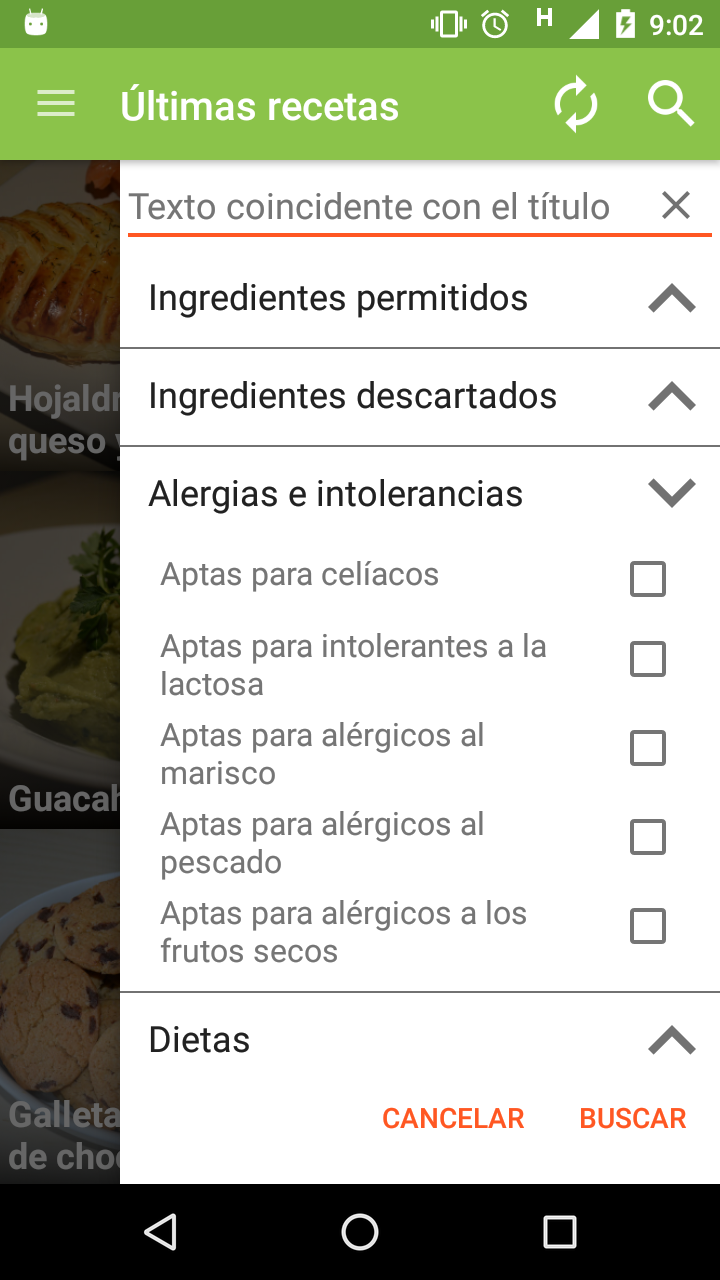
\includegraphics[width=\linewidth]{img/captura_06}
      \end{figure}
    \end{minipage}
    \hspace{0.05\linewidth}
    \begin{minipage}{0.4\linewidth}
      \begin{figure}[H]
        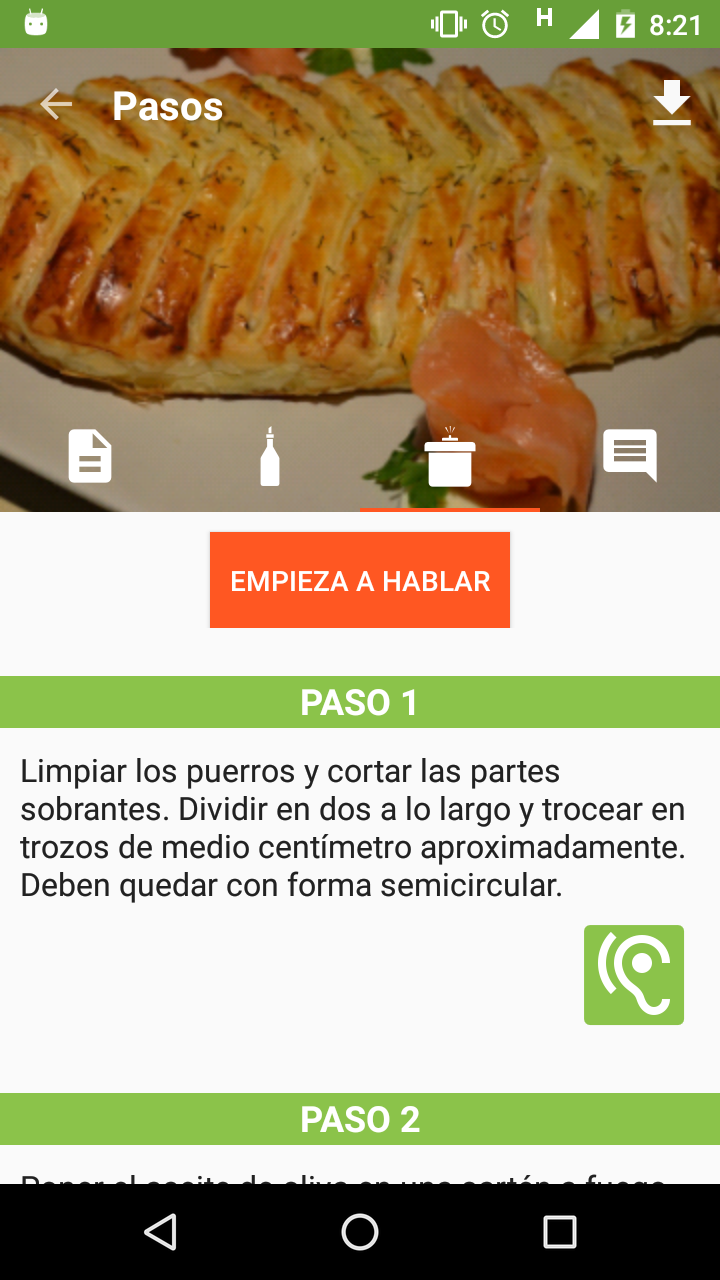
\includegraphics[width=\linewidth]{img/captura_11}
      \end{figure}
    \end{minipage}
  \end{minipage}
\end{frame}


\subsection{Desarrollo}

\begin{frame}{Tecnologías utilizadas}

  \begin{minipage}[t]{.6\textwidth}
    \begin{itemize}
    \item API:
      \begin{itemize}
      \item Python, Django, Django Rest Framework
      \item nginx, Gunicorn, Supervisor
      \item PostgreSQL
      \end{itemize}
    \item Aplicación móvil:
      \begin{itemize}
      \item SDK oficial
      \item Text To Speech
      \item Speech Recognizer
      \item Picasso, Retrofit
      \end{itemize}
    \item Otras:
      \begin{itemize}
      \item GNU Emacs, Android Studio
      \item Vagrant, Ansible
      \end{itemize}    
    \end{itemize}
  \end{minipage}%
  \begin{minipage}[t]{.4\textwidth}    
    \begin{figure}[H]
      \centering
      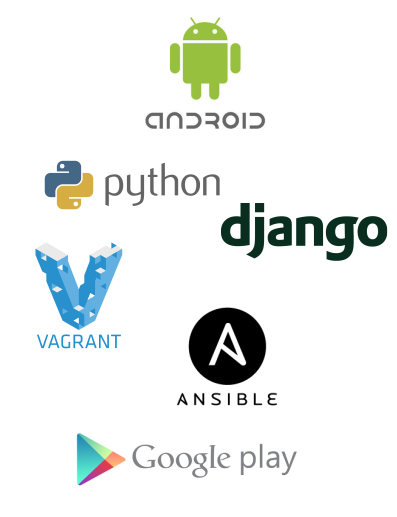
\includegraphics[width=\textwidth]{./img/nube-tecnologias}
    \end{figure}
  \end{minipage}
\end{frame}


\begin{frame}[fragile]{Implementación: Categorización}

  \begin{cambiarmargen}{-0.5cm}{-0.5cm}
    \textcolor{naranja}{\textsc{Idea original}}: Sistema automático de detección
    de alérgenos

    \begin{block}{DBpedia}
      Consulta sobre información semántica de datos de Wikipedia
    \end{block}

    
    \begin{minted}{bash}
PREFIX dcterms: <http://purl.org/dc/terms/>
select * where{
  ?marisco dcterms:subject
  <http://es.dbpedia.org/resource/Categoría:Marisco> .
}
    \end{minted}

    \vspace*{0.5cm}
    
    \then{} Información inconsistente: automatización imposible\\
    \then{} Peligro de obtener un falso positivo
  \end{cambiarmargen}
\end{frame}



\begin{frame}{Implementación: Categorización}

  \textcolor{naranja}{\textsc{Solución}}: \textit{Endpoint} de ingredientes
  categorizados en la API

  \begin{itemize}
  \item Intolerancia al gluten
  \item Intolerancia a la lactosa
  \item Alergia al marisco
  \item Alergia al pescado
  \item Alergia a los frutos secos
  \item \textbf{Sin categorizar}
  \end{itemize}
  
\end{frame}


\begin{frame}{Pruebas de software}

  \begin{block}{Entorno de testing}
    Desplegado con Vagrant y Ansible
    
    \begin{itemize}
    \item Plan de pruebas - Bloques funcionales
    \item Pruebas de seguridad
    \item Verificación de calidad del código
    \end{itemize}
  \end{block}
      
  \begin{block}{Entorno de producción real}
    Desde julio de 2016
    \begin{itemize}
    \item Play Store: Beta de la app
    \item Testers y dispositivos variados
    \end{itemize}
  \end{block}
  
\end{frame}


%% Conclusiones

\section{Conclusiones}

\subsection{Conclusiones}

\begin{frame}{Objetivos cumplidos}
  \begin{enumerate}
  \item Visualización de recetas
  \item Acceso público y compartir recetas
  \item Categorización y filtrado
  \item Multiidioma
  \item Lectura automática
  \item Captura de órdenes
  \end{enumerate}  
  
\end{frame}


\begin{frame}{Experiencia}
  He aprendido...
  \begin{itemize}
  \item a trabajar en plataformas Android
  \item algo más de Python (Django)
  \item a utilizar Vagrant
  \item despliegue de un proyecto real en Google Play
  \item muchas recetas nuevas
  \end{itemize}
\end{frame}  


\begin{frame}{Futuras ampliaciones}

  \begin{itemize}
  \item Unidades de medida dinámicas\\
    \then{} Multiplicador por comensales

    \vspace*{0.5cm}
  \item Calendario de comidas

    \vspace*{0.5cm}
  \item Listado de la compra
  \end{itemize}
\end{frame}


\begin{frame}{Demostración}

  \begin{center}
    \Huge Demostración
  \end{center}
\end{frame}  


\begin{frame}{Preguntas}

  \begin{center}
    \Large Gracias por su atención\\
    \vspace*{1cm}
    \large \url{https://github.com/nessa/serenity}\\
    \large \url{https://github.com/nessa/serenity-app}
  \end{center}
\end{frame}  

\licencia

\end{document}
